\def\lecturenumber{14}
\documentclass[11pt,a4paper]{article}
\usepackage[T1]{fontenc}
\usepackage[utf8]{inputenc}
\usepackage{lmodern}
\usepackage[margin=19mm,top=21mm,bottom=21mm,headheight=15pt]{geometry}
\usepackage{amsmath,amssymb,booktabs,array,graphicx,microtype}
\usepackage[dvipsnames]{xcolor}
\usepackage{enumitem,fancyhdr,listings,tcolorbox}
\usepackage[colorlinks=true,linkcolor=MidnightBlue,urlcolor=MidnightBlue]{hyperref}
\definecolor{courseblue}{HTML}{164B69}
\definecolor{pale}{HTML}{F0F5F7}
\pagestyle{fancy}
\fancyhf{}
\fancyhead[L]{\small\sffamily\color{courseblue}VALIDATED COMPUTING}
\fancyhead[R]{\small\sffamily Lecture \lecturenumber}
\fancyfoot[L]{\footnotesize Expanded lecture notes \textbullet\ October 2026}
\fancyfoot[R]{\footnotesize\thepage\ / 6}
\renewcommand{\headrulewidth}{0.4pt}
\setlength{\parindent}{0pt}
\setlength{\parskip}{5.5pt plus 1pt}
\setlength{\emergencystretch}{1.5em}
\setlist[itemize]{leftmargin=1.5em,itemsep=3pt,topsep=3pt}
\setlist[enumerate]{leftmargin=1.7em,itemsep=5pt,topsep=4pt}
\lstset{language=Python,basicstyle=\small\ttfamily,keywordstyle=\color{courseblue}\bfseries,
 commentstyle=\color{OliveGreen},stringstyle=\color{BrickRed},showstringspaces=false,
 columns=fullflexible,keepspaces=true,frame=single,rulecolor=\color{black!18},
 backgroundcolor=\color{black!2},aboveskip=6pt,belowskip=6pt,breaklines=true,
 xleftmargin=5pt,xrightmargin=5pt,framesep=5pt}
\newcommand{\R}{\mathbb R}
\newcommand{\fl}{\operatorname{fl}}
\newcommand{\abs}[1]{\left|#1\right|}
\newcommand{\heading}[2]{\section*{\color{courseblue}#1}\vspace{-4pt}{\small\sffamily\color{black!65}#2}\par\vspace{3pt}}
\newcommand{\opening}[2]{{\Large\sffamily\bfseries\color{courseblue}Lecture \lecturenumber\quad #1\par}\vspace{5pt}{\small #2}\par}
\newtcolorbox{question}[1]{colback=pale,colframe=courseblue!55,boxrule=0.4pt,
 arc=1mm,left=7pt,right=7pt,top=4pt,bottom=4pt,title={#1},fonttitle=\bfseries\small,
 coltitle=courseblue,colbacktitle=pale}
\newcommand{\reading}[1]{{\footnotesize\textbf{Reading and notebook.} #1\par}}
\hypersetup{pdfauthor={Validated Computing course},pdfsubject={Expanded introductory lecture notes with questions and exercises}}

\hypersetup{pdftitle={Lecture 14: From numerical experiments to supported claims}}
\begin{document}
\opening{From numerical experiments to supported claims}{Prerequisites: the completed introductory sequence and a prepared project example.\newline
Goal: choose an appropriate validation argument, explain its limits, and present a reproducible, accurately scoped result.}
\heading{1. Match the method to the missing argument}{0--12 minutes: connect the course's different guarantees}
The course began with computations that looked plausible but did not
establish the intended answer. We now have several ways to strengthen a
result. The first step is still to name the claim: a good approximation,
an enclosure of every allowed value, exactly one root in a region, or an
account of all relevant solutions on a domain.

These claims are not interchangeable. A function enclosure that contains
zero need not contain an actual root value. A local uniqueness certificate
does not exclude roots elsewhere. An exact minimum value does not identify
all minimizing locations. A completed event sequence must reach the requested
time before its endpoint can be reported there.

\begin{center}
\begin{tabular}{p{0.31\linewidth}p{0.59\linewidth}}
\toprule
Obstacle & A response that addresses it\\
\midrule
Arithmetic rounding & Use exact arithmetic or outward rounding; increase
precision when enclosure widths are dominated by rounding.\\[4pt]
Cancellation or dependency & Reformulate the expression, preserve a useful
relation, or subdivide while retaining a valid cover.\\[4pt]
Unknown existence or uniqueness & Supply a theorem with verified premises,
such as strict interval Newton inclusion.\\[4pt]
Unsettled global scope & Account for every relevant region or event;
retain unresolved work explicitly.\\[4pt]
Uncertain physical inputs & Enclose the whole allowed family and report
which claims hold uniformly over it.\\
\bottomrule
\end{tabular}
\end{center}

\textbf{Three compact examples.} Exact rational evaluation proves that the
orientation example with $n=2^{27}$ has determinant one, despite a binary64
zero. Interval Newton on $x^2-2$ over $[1,2]$ gives
$[11/8,23/16]\subset(1,2)$, proving a unique root in the stated domain.
For $(x^2-1)^2$ on $[-2,2]$, nonnegativity and the feasible point $1$
prove minimum value zero; the second minimizer at $-1$ still matters to a
claim about every minimizing location.

\begin{question}{Choose a repair before choosing a precision}
A root search has narrow certified boxes but one unresolved region. A
determinant bound is too wide to decide its sign for exact input points.
Which problem might more bits address directly, and which still needs a
coverage decision? State what evidence would show the repair succeeded.
\end{question}

The common structure is a stated input model, a valid inclusion argument,
a theorem or decision rule, and an honest description of scope. The next
example exposes another source of excess width that remains even when all
arithmetic is exact: repeatedly forgetting the shape of a set.

\newpage
\heading{2. Wrapping can grow without any rounding error}{12--27 minutes: rotate a square and inspect the lost relation}
Consider the exact rational matrix
\[
 Q=\begin{pmatrix}3/5&-4/5\\4/5&3/5\end{pmatrix}.
\]
Its columns have squared length $9/25+16/25=1$ and dot product zero;
its determinant is one. Thus $Q^TQ=I$, so it is a rotation and preserves
Euclidean lengths. Begin with the square $S_0=[-1,1]^2$.

One interval matrix multiplication gives a coordinate box
$B_1=[-7/5,7/5]^2$. This is exactly the smallest axis-aligned box
containing the rotated square $QS_0$. Nevertheless, the square and its
box are different sets. In the box, coordinates can vary independently;
in the rotated square, some combinations of coordinates are impossible.

If we rotate the \emph{box} again, the new coordinate radius is multiplied
by $|3/5|+|4/5|=7/5$. Repeating the procedure gives
\[
               B_k=[-(7/5)^k,(7/5)^k]^2,
 \qquad \operatorname{width}_x(B_k)=2(7/5)^k.
\]
Every $B_k$ encloses the actual rotated square $Q^kS_0$, but the repeated
replacement by boxes introduces artificial combinations at each step.
This is the \emph{wrapping effect}.

\textbf{Compare the second step exactly.} Direct multiplication gives
\[
 Q^2=\begin{pmatrix}-7/25&-24/25\\24/25&-7/25\end{pmatrix}.
\]
Its true coordinate widths on $S_0$ are $2(7/25+24/25)=62/25$.
Repeated box propagation instead gives $2(7/5)^2=98/25$. Both calculations
use exact rational arithmetic. Their discrepancy is a representation loss,
so adding arithmetic bits cannot remove it.

More generally, write
$Q^k=\left(\begin{smallmatrix}a_k&-b_k\\b_k&a_k\end{smallmatrix}\right)$,
with $a_k^2+b_k^2=1$. The true coordinate width is
$2(|a_k|+|b_k|)$. Since $1\le |a_k|+|b_k|\le\sqrt2$, this width always
lies between $2$ and $2\sqrt2$, however many rotations are applied.
The exponentially growing box width therefore does not describe physical
growth of the original set.

\begin{question}{Which operation loses the information?}
At the first step, are the coordinate bounds already wrong? Which points
are introduced when the rotated square is replaced by a box? Why can a
perfectly sharp one-step enclosure still cause excess width after repetition?
\end{question}

Preserving a polygon, using better coordinates, or subdividing the input
can reduce wrapping, at a computational cost. For this linear example the
four exact vertices are enough. A nonlinear image generally needs more
information than simply evaluating its original corners.

\newpage
\heading{3. Compare two exact computations in readable Python}{27--42 minutes: store the corners as well as the box radius}
A linear functional on a square reaches its extrema at vertices. Thus
rotating all four vertices computes the true coordinate range here. Run
this standalone code with Python's standard library; floats are used only
by the separate figure-generation code when drawing the results.
\begin{lstlisting}
from fractions import Fraction

c, s = Fraction(3, 5), Fraction(4, 5)
corners = []
for x in [-1, 1]:
    for y in [-1, 1]:
        corners.append((Fraction(x), Fraction(y)))
radius = Fraction(1)
box_widths, true_widths = [], []
for step in range(16):
    x_values = []
    for x, y in corners:
        x_values.append(x)
    true_width = max(x_values) - min(x_values)
    box_width = 2 * radius
    assert true_width <= box_width
    assert 4 <= true_width*true_width <= 8
    box_widths.append(box_width)
    true_widths.append(true_width)
    new_corners = []
    for x, y in corners:
        new_corners.append((c*x-s*y, s*x+c*y))
    corners = new_corners
    radius = (abs(c) + abs(s)) * radius
assert box_widths[2] == Fraction(98, 25)
assert true_widths[2] == Fraction(62, 25)
\end{lstlisting}

\begin{center}
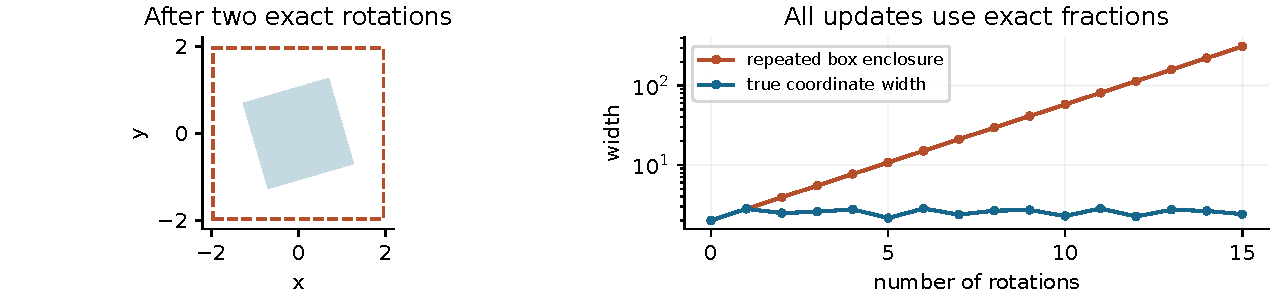
\includegraphics[width=0.92\linewidth]{figures/exact_wrapping.pdf}
\end{center}

The assertions compare exact fractions. Squaring the positive true width
allows the bound $2\sqrt2$ to be checked without approximating that square
root. The graph illustrates the result; the orthogonality and vertex
arguments explain why it holds for the entire input square.

\begin{question}{Read the graph without changing the claim}
Does the rising curve prove that nearby exact trajectories separate
exponentially? Which curve follows the actual set? Explain why plotting
floating-point versions of exact widths does not make the plot the proof.
\end{question}

\newpage
\heading{4. Separate precision, input sensitivity, and event ambiguity}{42--58 minutes: interpret a mirror experiment carefully}
The mirror project combines several sources of difficulty. Rounding may
widen the arithmetic bounds. Repeated enclosure operations may lose
relations among position, direction, and collision time. A genuinely uncertain
initial condition describes several possible trajectories. An event decision
may remain ambiguous even when each candidate time is accurately bounded.
These effects require different interpretations and sometimes different remedies.

\textbf{Two distinct experiments.} First keep the exact initial data fixed
and increase arithmetic precision. Record whether the same time horizon is
certified, the event decisions, and the output widths. Second, keep the
arithmetic procedure fixed and deliberately vary or enclose an initial
coordinate. This changes the mathematical problem. Extra precision cannot
remove variation that belongs to the allowed family of inputs.

A single-circle calculation already shows geometric sensitivity. For an
eastward ray starting at $(1/2,y)$ and a circle centred at $(1,0)$ with
radius $r=1/3$, the entry time for $|y|<r$ is
\[
             t(y)=\frac12-\sqrt{r^2-y^2},\qquad
             t'(y)=\frac{y}{\sqrt{r^2-y^2}}.
\]
The derivative grows without bound as $y\to r$ from below. At tangency
the branch structure changes: the two intersection times coalesce, and
for $|y|>r$ this circle is missed. This is a local geometric explanation
of sensitivity near grazing, not a proof of chaotic dynamics in the
entire mirror system.

At the standard height $y=1/10$, this candidate time is
$1/2-\sqrt{91}/30$. A simulation of the full lattice must additionally
prove that this candidate is the first event among all reachable mirrors.
Accurately computing a reflection from one chosen circle does not settle
that ordering question.

\begin{question}{Diagnose an unresolved run before changing it}
A computation reports overlapping time enclosures for two candidate hits.
What would justify increasing precision? What evidence could instead show
that the input family permits different first hits? What remains valid if
the run can report only its last certified state?
\end{question}

The introductory project asks for the exact standard input at time three,
with coordinate and distance widths at most $10^{-20}$. The original SIAM
time-ten challenge is an extension, not a condition for completing this
course. A longer horizon may accumulate more rounding, dependency loss,
and difficult event decisions. Compare completion and accuracy separately.

The rotation example also warns against diagnosing physical instability
from a growing enclosure alone. Use exact-model arguments, controlled input
changes, and certified comparisons to distinguish actual sensitivity from
artifacts of the representation. A striking visualization can suggest a
question; it does not decide which mechanism produced the observed behavior.

\newpage
\heading{5. Present a project as a claim with inspectable evidence}{58--80 minutes: two short demonstrations and a shared review}
Use two eight-minute demonstrations followed by six minutes of discussion.
For a larger class, continue demonstrations in another session or collect
recorded presentations; the six-page notes do not imply that every project
can be heard in one meeting. Prepare a fresh-kernel run beforehand and
retain its data, so live execution problems do not obscure the mathematical review.

An eight-minute presentation can follow this sequence:
\begin{enumerate}
\item \textbf{One minute: specify the question.} State the exact inputs
or uncertainty set, domain or final time, and desired conclusion. Distinguish
value accuracy from location accuracy and local scope from global scope.
\item \textbf{One minute: show the exploration.} Explain how approximate
calculations suggested a candidate. Label plotted or printed approximations
as such. Identify what this exploratory stage did not yet prove.
\item \textbf{Three minutes: show the validation argument.} Name the
theorem or invariant and display the decisive bounds. Explain one
nontrivial premise, branch decision, or coverage record rather than reading
every line of code aloud.
\item \textbf{Two minutes: show a limitation and a correction.} Present
one inconclusive case and its honest output. Describe a concrete peer-audit
finding, the response, and any change to the supported claim.
\item \textbf{One minute: state the result.} Give the exact certificate
location, reproduction information, and the final mathematical conclusion,
including any unresolved scope or unmet target.
\end{enumerate}

For example, a root presentation could begin with an approximate $\sqrt2$,
then show $D=[2,4]$ and $N=[11/8,23/16]\subset(1,2)$. It should explain
why the theorem proves existence and uniqueness and why the conclusion is
local. A double-root or boundary-root example can demonstrate an honest
failure of the taught strict test. A screenshot of a long decimal expansion
would leave most of this argument unavailable to the audience.

\begin{center}
\begin{tabular}{p{0.73\linewidth}r}
\toprule
Project rubric component & Weight\\
\midrule
Precise claim and input model & 20\%\\
Mathematical validation argument & 30\%\\
Readable implementation and evidence & 25\%\\
Reproduction and interpretation & 15\%\\
Audit response and presentation & 10\%\\
\bottomrule
\end{tabular}
\end{center}

These weights reproduce the capstone rubric, not the weighting of the
whole course. Submit the completed notebook, certificate data where
applicable, and the peer audit with the author's responses. A precisely
bounded partial result can be valuable; a success claim that omits a
missing hypothesis or unresolved region is unsupported.

\begin{question}{An audience question that tests the argument}
Ask which recorded bound establishes the central conclusion and which
assumption that bound relies on. Then ask what would remain true if the
budget ended earlier. Evaluate the answer's scope rather than the number
of digits displayed.
\end{question}

\newpage
\heading{6. Final exercises and directions for further study}{80--90 minutes: discuss two claims; retain the rest for review}
\begin{enumerate}
\item \textbf{Wrapping without rounding.} Compute $Q^2$ and the two
second-step widths from pages 2--3. Explain why the true width remains
bounded for every number of rotations. Would evaluating only four corners
also bound the range of an arbitrary nonlinear map on the square?

\item \textbf{Agreement is evidence.} Two nearest-rounded computations
at different precisions agree to ten decimal places. What has not yet been
established? State a possible rigorous replacement claim involving a common
exact input and enclosing endpoints.

\item \textbf{A zero gap and a wide set.} The objective is identically
three on $[-10,10]$. Give its minimum value and complete minimizer set.
Explain why a correct optimization result may have zero value gap and a
candidate domain of width 20.

\item \textbf{A zero residual and two roots.} For
$g(x,y)=(x+y,x+(1+\varepsilon)y+x^2)$, $\varepsilon>0$, verify the two
roots $(0,0)$ and $(\varepsilon,-\varepsilon)$. What is wrong with
inferring local-box uniqueness from the residual at the origin alone?

\item \textbf{Choose the next valid claim.} A root search or trajectory
run retains explicit unresolved work. Write one useful partial claim and
one stronger claim that would require more evidence. State whether more
precision, a larger search budget, or a revised input model addresses the
particular obstruction you chose.
\end{enumerate}

\textbf{Selected checks.} Exercise 1 gives true width $62/25$ and repeated
box width $98/25$; orthogonality bounds true widths by $2\sqrt2$.
Corners alone are insufficient for a general nonlinear map: for example,
$x^2+y^2$ is two at every vertex of $[-1,1]^2$ but zero at the centre.
Exercise 2 lacks a one-sided or all-input error argument; enclosing the
exact quantity within a sufficiently narrow interval can supply one.
Exercise 3 has minimum three at every point of the domain. Exercise 4
reduces to $y=-x$ and $x(x-\varepsilon)=0$; a box containing both roots
cannot have a valid uniqueness certificate. In Exercise 5, retain the
recorded domain, time, and status in the partial conclusion.

\begin{question}{Final exit ticket: complete the sentence with evidence}
``Under these input and model assumptions, the computation proves\ldots''
Name the enclosure or theorem that closes the argument, the relevant
domain or final time, and any unresolved part. Identify one feature of
the implementation that a reviewer must still trust or inspect.
\end{question}

Further topics extend different parts of this argument. Taylor models
retain functional dependence together with a remainder enclosure. Verified
integration and ODE methods add bounds for discretization and truncation.
Higher-dimensional searches need scalable representations and coverage
arguments. Formal proof assistants address explicit verification of proof
steps, with their own implementation and trusted-kernel questions. These
are extensions beyond the algorithms developed in this introduction.

\reading{Companion: \texttt{notebooks/14\_synthesis.ipynb}; project rubric:
\texttt{projects/README.md}. Revisit Lectures 01--13 as needed. For the mirror
motivation, see SIAM Challenge Chapter 2, especially \S2.3. The local
advanced-course review in \texttt{Doc/existing\_course\_review.md} describes
possible later study and its additional prerequisites.}
\end{document}
